\documentclass{article}
\usepackage[utf8]{inputenc}
\usepackage[english]{babel}
 \usepackage{graphicx}
 \usepackage{float}
 \graphicspath{ {} }
 \usepackage{mathtools}
 \usepackage{amsmath, amsthm, amssymb, amsfonts}
 \usepackage{caption}
 \usepackage{titlepic}
\usepackage{hyperref}
\hypersetup{
    colorlinks=true,
    linkcolor=blue,
    filecolor=magenta,      
    urlcolor=cyan,
    pdftitle={Probability Notes},
    pdfauthor={Ty Darnell},
    bookmarksopen=true,
}
\numberwithin{equation}{section}

\begin{document}
\begin{flushleft}
\begin{figure}[H]
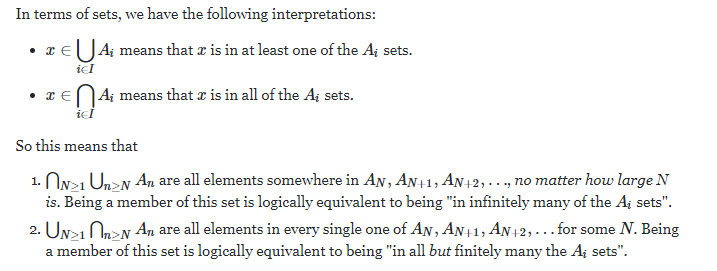
\includegraphics[scale=.8]{infsup.png}
\end{figure}
\medbreak
\textbf{Lim inf}
\begin{figure}[H]
	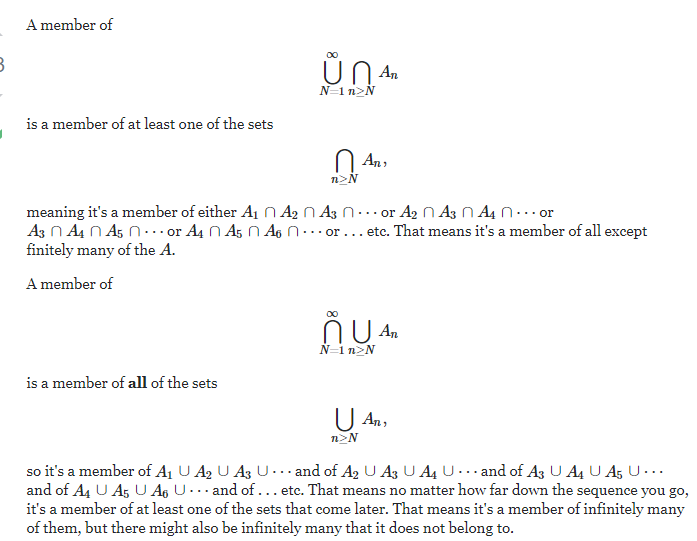
\includegraphics[scale=.8]{liminfexplained.png}
\end{figure}






\end{flushleft}
\end{document}
